\documentclass[]{standalone}

\usepackage{graphicx}

\usepackage{tikz}

\usetikzlibrary{positioning}
\usetikzlibrary{arrows.meta}
\usetikzlibrary{calc}

\begin{document}

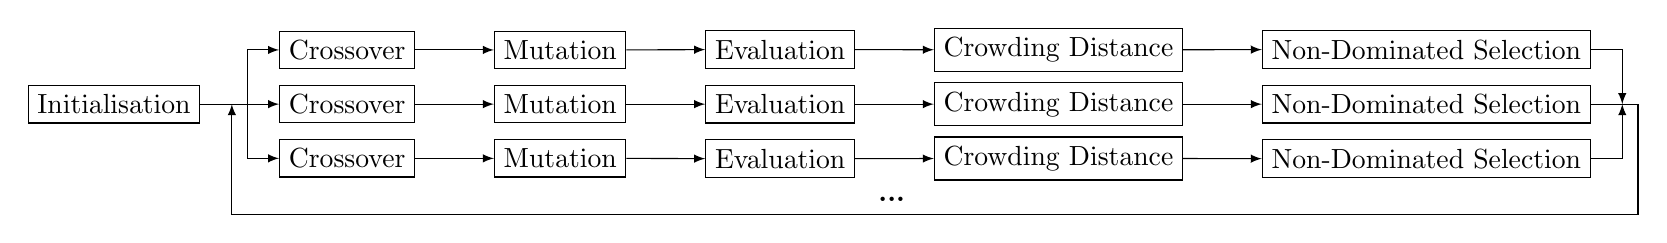
\begin{tikzpicture}[
    block/.style={rectangle, draw=black, fill=white},
]
    \node[block] (B1) [] {Initialisation};

    \node[block] (BA2) [right=of B1] {Crossover};
    \node[block] (BA3) [right=of BA2] {Mutation};
    \node[block] (BA4) [right=of BA3] {Evaluation};
    \node[block] (BA5) [right=of BA4] {Crowding Distance};
    \node[block] (BA6) [right=of BA5] {Non-Dominated Selection};

    \node[block] (BB2) [above=0.2cm of BA2] {Crossover};
    \node[block] (BB3) [above=0.2cm of BA3] {Mutation};
    \node[block] (BB4) [above=0.2cm of BA4] {Evaluation};
    \node[block] (BB5) [above=0.13cm of BA5] {Crowding Distance};
    \node[block] (BB6) [above=0.2cm of BA6] {Non-Dominated Selection};

    \node[block] (BC2) [below=0.2cm of BA2] {Crossover};
    \node[block] (BC3) [below=0.2cm of BA3] {Mutation};
    \node[block] (BC4) [below=0.2cm of BA4] {Evaluation};
    \node[block] (BC5) [below=0.13cm of BA5] {Crowding Distance};
    \node[block] (BC6) [below=0.2cm of BA6] {Non-Dominated Selection};

    \node[] (H1) [below=0.15cm of BC4] {};
    \node[] (T1) [right=1cm of H1] {\textbf{...}};

    \draw[] (B1.east) -- ($(B1.east)+(0.6,0)$);
    \draw[-latex] ($(B1.east)+(0.6,0)$) -| ($(BA2.west)+(-0.4,0)$) -- (BA2.west);
    \draw[-latex] ($(B1.east)+(0.6,0)$) -| ($(BB2.west)+(-0.4,0)$) -- (BB2.west);
    \draw[-latex] ($(B1.east)+(0.6,0)$) -| ($(BC2.west)+(-0.4,0)$) -- (BC2.west);

    \draw[-latex] (BA2.east) -- (BA3.west);
    \draw[-latex] (BA3.east) -- (BA4.west);
    \draw[-latex] (BA4.east) -- (BA5.west);
    \draw[-latex] (BA5.east) -- (BA6.west);

    \draw[-latex] (BB2.east) -- (BB3.west);
    \draw[-latex] (BB3.east) -- (BB4.west);
    \draw[-latex] (BB4.east) -- (BB5.west);
    \draw[-latex] (BB5.east) -- (BB6.west);

    \draw[-latex] (BC2.east) -- (BC3.west);
    \draw[-latex] (BC3.east) -- (BC4.west);
    \draw[-latex] (BC4.east) -- (BC5.west);
    \draw[-latex] (BC5.east) -- (BC6.west);

    \draw[] (BA6.east) -| ($(BA6.east)+(0.4,0)$);
    \draw[-latex] (BB6.east) -| ($(BA6.east)+(0.4,0)$);
    \draw[-latex] (BC6.east) -| ($(BA6.east)+(0.4,0)$);

    \draw[-latex] ($(BA6.east)+(0.4,0)$) -| ($(BA6.east)+(0.6,-1.4)$) -| ($(B1.east)+(0.4,-1.4)$) -- ($(B1.east)+(0.4,0)$);
\end{tikzpicture}

\end{document}